\section{The Incidence Matrices and Hodge Matrices}

The incidence matrices, $\mathbb{E}$, and the Hodge matrices, $\mathbb{H}$, will be derived using the mesh introduced in the preceding section. In fact, the incidence and Hodge matrices derived in this section are only valid for the mesh shown in Figures \ref{fig:outerGrid} and \ref{fig:innerGrid}. That is, the validity is limited to the rather coarse spacing of $n = 3$. However, the format of those matrices belonging to denser grids can be correctly deduced by careful analysis of the matrix structure at $n = 3$, which is of course what we are after.

\subsection{$\tilde{\mathbb{E}}^{(2,1)}$}

Application of the incidence matrix $\tilde{\mathbb{E}}^{(2,1)}$ to line segments that represent mass flow, $\mathbf{\tilde{u}}^{(1)}$, yields the rate of mass production in the surface enclosed by those line segments, $\mathbf{\tilde{s}}^{(2)}$. This implies that
\begin{equation}
    \tilde{\mathbb{E}}^{(2,1)} \mathbf{\tilde{u}}^{(1)} = 0
\end{equation}
reads as conversation of mass; mass cannot be created nor destoryed and mass that flows into a surface, must flow out, and vice versa. Let us construct a linear equation for each of the surfaces $\tilde{s}_{(i,j)}$:
\begin{equation}
    \begin{split}
        \tilde{s}_{0,0} &= -\tilde{u}_{0,0} + \tilde{u}_{1,0} - \tilde{v}_{0,0} + \tilde{v}_{0,1} \\
        \tilde{s}_{1,0} &= -\tilde{u}_{1,0} + \tilde{u}_{2,0} - \tilde{v}_{1,0} + \tilde{v}_{1,1} \\
        &\vdots \\
        \tilde{s}_{2,2} &= -\tilde{u}_{2,2} + \tilde{u}_{3,2} - \tilde{v}_{2,2} + \tilde{v}_{2,3} \\
    \end{split}
    \label{eq:tsijEquations}
\end{equation}
Equation \eqref{eq:tsijEquations} expressed in matrix notation becomes
\begin{equation}
    \mathbf{\tilde{s}}^{(2)} = \tilde{\mathbb{E}}^{(2,1)} \mathbf{\tilde{u}}^{(1)}
    \label{eq:tE21}
\end{equation}
The mass flow rates $\tilde{u}_{(i,j)}$ and $\tilde{v}_{(i,j)}$ adjacent to the boundary of the unit square are known because the boundary conditions of the problem are known. The matrices in the right-hand side of Equation \eqref{eq:tE21} can be split into a matrix of unknowns and into a matrix of knows. Splitting the matrix yields
\begin{equation}
    \mathbf{\tilde{s}}^{(2)} = \tilde{\mathbb{E}}^{(2,1)} \mathbf{\tilde{u}}^{(1)} + \tilde{\mathbb{E}}^{(2,1)}_{\text{known}} \mathbf{\tilde{u}}^{(1)}_{\text{known}}
\end{equation}
where
\begin{flalign}
    & &
    \setlength{\arraycolsep}{-0.5pt}
    \tilde{\mathbb{E}}^{(2,1)} =
    \left[
    \begin{array}{cccccccccccc}
        \w{1} & \d & \d & \d & \d & \d & \w{1} & \d & \d & \d & \d & \d \\
        -1 & \w{1} & \d & \d & \d & \d & \d & \w{1} & \d & \d & \d & \d \\
        \d & -1 & \d & \d & \d & \d & \d & \d & \w{1} & \d & \d & \d \\
        \d & \d & \w{1} & \d & \d & \d & -1 & \d & \d & \w{1} & \d & \d \\
        \d & \d & -1 & \w{1} & \d & \d & \d & -1 & \d & \d & \w{1} & \d \\
        \d & \d & \d & -1 & \d & \d & \d & \d & -1 & \d & \d & \w{1} \\
        \d & \d & \d & \d & \w{1} & \d & \d & \d & \d & -1 & \d & \d \\
        \d & \d & \d & \d & -1 & \w{1} & \d & \d & \d & \d & -1 & \d \\
        \d & \d & \d & \d & \d & -1 & \d & \d & \d & \d & \d & -1 \\
    \end{array}
    \right] && \\
    & \text{and} &
    \setlength{\arraycolsep}{-0.5pt}
    \tilde{\mathbb{E}}^{(2,1)}_{\text{known}} =
    \left[
    \begin{array}{cccccccccccc}
        -1 & \d & \d & \d & \d & \d & -1 & \d & \d & \d & \d & \d \\
        \d & \d & \d & \d & \d & \d & \d & -1 & \d & \d & \d & \d \\
        \d & \w{1} & \d & \d & \d & \d & \d & \d & -1 & \d & \d & \d \\
        \d & \d & -1 & \d & \d & \d & \d & \d & \d & \d & \d & \d \\
        \d & \d & \d & \d & \d & \d & \d & \d & \d & \d & \d & \d \\
        \d & \d & \d & \w{1} & \d & \d & \d & \d & \d & \d & \d & \d \\
        \d & \d & \d & \d & -1 & \d & \d & \d & \d & \w{1} & \d & \d \\
        \d & \d & \d & \d & \d & \d & \d & \d & \d & \d & \w{1} & \d \\
        \d & \d & \d & \d & \d & \w{1} & \d & \d & \d & \d & \d & \w{1} \\
    \end{array}
    \right] &&
\end{flalign}

\subsection{$\mathbb{E}^{(1,0)}$}

The incidence matrix $\mathbb{E}^{(1,0)}$ maps an inner-oriented 0-cochain to an inner-oriented 1-cochain. Let us create a linear equation for each of the 1-cells, $u_{(i,j)}$, in the inner-oriented grid, considering that the 0-cells, $P_{(i,j)}$, are sink-like. The equations are
\begin{equation}
    \begin{split}
        u_{1,1} &= -p_{1,1} + p_{2,1} \\
        u_{2,1} &= -p_{2,1} + p_{3,1} \\
        &\vdots \\
        u_{2,3} &= -p_{2,3} + p_{3,3} \\
        v_{1,1} &= -p_{1,1} + p_{1,2} \\
        v_{2,1} &= -p_{2,1} + p_{2,2} \\
        &\vdots \\
        v_{3,2} &= -p_{3,2} + p_{3,3}
    \end{split}
    \label{eq:E10list}
\end{equation}
Equation \eqref{eq:E10list} can be written in matrix notation as
\begin{equation}
    \mathbf{u} = \mathbb{E}^{(1,0)} \mathbf{p}
\end{equation}
where
\begin{equation}
    \setlength{\arraycolsep}{-0.5pt}
    \mathbb{E}^{(1,0)} =
    \left[
    \begin{array}{ccccccccc}
        -1 & \w{1} & \d & \d & \d & \d & \d & \d & \d \\
        \d & -1 & \w{1} & \d & \d & \d & \d & \d & \d \\
        \d & \d & \d & -1 & \w{1} & \d & \d & \d & \d \\
        \d & \d & \d & \d & -1 & \w{1} & \d & \d & \d \\
        \d & \d & \d & \d & \d & \d & -1 & \w{1} & \d \\
        \d & \d & \d & \d & \d & \d & \d & -1 & \w{1} \\
        -1 & \d & \d & \w{1} & \d & \d & \d & \d & \d \\
        \d & -1 & \d & \d & \w{1} & \d & \d & \d & \d \\
        \d & \d & -1 & \d & \d & \w{1} & \d & \d & \d \\
        \d & \d & \d & -1 & \d & \d & \w{1} & \d & \d \\
        \d & \d & \d & \d & -1 & \d & \d & \w{1} & \d \\
        \d & \d & \d & \d & \d & -1 & \d & \d & \w{1}
    \end{array}
    \right]
\end{equation}

It is important to notice that
\begin{equation}
    \mathbb{E}^{(1,0)} = -\left(\tilde{\mathbb{E}}^{(2,1)}\right)^T
\end{equation}

\subsection{$\mathbb{E}^{(2,1)}$}

The incidence matrix $\mathbb{E}^{(2,1)}$ maps an inner-oriented 1-cochain to an inner-oriented 2-cochain. That is, it maps circulation along line segments to vorticity in the planes enclosed by those line segments. The derivation of $\mathbb{E}^{(2,1)}$ is straightforward: add the circulation along those line segments sharing a common orientation with the plane and subtract the circulation along those line segments whose orientation opposes the orientation of the plane. Executing this procedure for all planes $\xi_{i,j}$, we have
\begin{equation}
    \begin{split}
        \mathbf{\xi}_{0,0} &= u_{0,0} - u_{0,1} - v_{0,0} + v_{1,0} \\
        \mathbf{\xi}_{1,0} &= u_{1,0} - u_{1,1} - v_{1,0} + v_{2,0} \\
        &\vdots \\
        \mathbf{\xi}_{3,3} &= u_{3,3} - u_{3,4} - v_{3,3} + v_{4,3}
    \end{split}
\end{equation}
which is in accordance to the formula
\begin{equation}
    \xi_{i,j} = u_{i,j} - u_{i,j+1} - v_{i,j} + v_{i+1,j}
\end{equation}

\begin{equation}
    \mathbf{\xi}^{(2)} = \mathbb{E}^{(2,1)} \mathbf{u}^{(1)}
\end{equation}

The velocities adjacent to the boundary are again known because the boundary conditions of the problem are known. In a similar fashion as in Section 3.9.1, splitting the incidence matrix $\mathbb{E}^{(2,1)}$ into a matrix of unknowns and into a matrix of knows, we have
\begin{equation}
    \mathbf{\xi}^{(2)} = \mathbb{E}^{(2,1)} \mathbf{u}^{(1)} + \mathbb{E}^{(2,1)}_{\text{known}} \mathbf{u}^{(1)}_{\text{known}}
\end{equation}
where
\begin{equation}
    \setlength{\arraycolsep}{-0.5pt}
    \mathbb{E}^{(2,1)} =
    \left[
    \begin{array}{cccccccccccc}
        \d & \d & \d & \d & \d & \d & \d & \d & \d & \d & \d & \d \\
        -1 & \d & \d & \d & \d & \d & \d & \d & \d & \d & \d & \d \\
        \d & -1 & \d & \d & \d & \d & \d & \d & \d & \d & \d & \d \\
        \d & \d & \d & \d & \d & \d & \d & \d & \d & \d & \d & \d \\
        \d & \d & \d & \d & \d & \d & \w{1} & \d & \d & \d & \d & \d \\
        \w{1} & \d & -1 & \d & \d & \d & -1 & \w{1} & \d & \d & \d & \d \\
        \d & \w{1} & \d & -1 & \d & \d & \d & -1 & \w{1} & \d & \d & \d \\
        \d & \d & \d & \d & \d & \d & \d & \d & -1 & \d & \d & \d \\
        \d & \d & \d & \d & \d & \d & \d & \d & \d & \w{1} & \d & \d \\
        \d & \d & \w{1} & \d & -1 & \d & \d & \d & \d & -1 & \w{1} & \d \\
        \d & \d & \d & \w{1} & \d & -1 & \d & \d & \d & \d & -1 & \w{1} \\
        \d & \d & \d & \d & \d & \d & \d & \d & \d & \d & \d & -1 \\
        \d & \d & \d & \d & \d & \d & \d & \d & \d & \d & \d & \d \\
        \d & \d & \d & \d & \w{1} & \d & \d & \d & \d & \d & \d & \d \\
        \d & \d & \d & \d & \d & \w{1} & \d & \d & \d & \d & \d & \d \\
        \d & \d & \d & \d & \d & \d & \d & \d & \d & \d & \d & \d
    \end{array}
    \right]
\end{equation}
and
\begin{multline}
    \mathbb{E}^{(2,1)}_{\text{known}} = \\
    \setlength{\arraycolsep}{-0.5pt}
    \left[
    \begin{array}{cccccccccccccccccccccccccccc}
        \w{1} & \d & \d & \d & -1 & \d & \d & \d & \d & \d & \d & \d & \d & \d &
        -1 & \w{1} & \d & \d & \d & \d & \d & \d & \d & \d & \d & \d & \d & \d \\
        \d & \w{1} & \d & \d & \d & \d & \d & \d & \d & \d & \d & \d & \d & \d &
        \d & -1 & \w{1} & \d & \d & \d & \d & \d & \d & \d & \d & \d & \d & \d \\
        \d & \d & \w{1} & \d & \d & \d & \d & \d & \d & \d & \d & \d & \d & \d &
        \d & \d & -1 & \w{1} & \d & \d & \d & \d & \d & \d & \d & \d & \d & \d \\
        \d & \d & \d & \w{1} & \d & -1 & \d & \d & \d & \d & \d & \d & \d & \d &
        \d & \d & \d & -1 & \w{1} & \d & \d & \d & \d & \d & \d & \d & \d & \d \\
        \d & \d & \d & \d & \w{1} & \d & -1 & \d & \d & \d & \d & \d & \d & \d &
        \d & \d & \d & \d & \d & -1 & \d & \d & \d & \d & \d & \d & \d & \d \\
        \d & \d & \d & \d & \d & \d & \d & \d & \d & \d & \d & \d & \d & \d &
        \d & \d & \d & \d & \d & \d & \d & \d & \d & \d & \d & \d & \d & \d \\
        \d & \d & \d & \d & \d & \d & \d & \d & \d & \d & \d & \d & \d & \d &
        \d & \d & \d & \d & \d & \d & \d & \d & \d & \d & \d & \d & \d & \d \\
        \d & \d & \d & \d & \d & \w{1} & \d & -1 & \d & \d & \d & \d & \d & \d &
        \d & \d & \d & \d & \d & \d & \w{1} & \d & \d & \d & \d & \d & \d & \d \\
        \d & \d & \d & \d & \d & \d & \w{1} & \d & -1 & \d & \d & \d & \d & \d &
        \d & \d & \d & \d & \d & \d & \d & -1 & \d & \d & \d & \d & \d & \d \\
        \d & \d & \d & \d & \d & \d & \d & \d & \d & \d & \d & \d & \d & \d &
        \d & \d & \d & \d & \d & \d & \d & \d & \d & \d & \d & \d & \d & \d \\
        \d & \d & \d & \d & \d & \d & \d & \d & \d & \d & \d & \d & \d & \d &
        \d & \d & \d & \d & \d & \d & \d & \d & \d & \d & \d & \d & \d & \d \\
        \d & \d & \d & \d & \d & \d & \d & \w{1} & \d & -1 & \d & \d & \d & \d &
        \d & \d & \d & \d & \d & \d & \d & \d & \w{1} & \d & \d & \d & \d & \d \\
        \d & \d & \d & \d & \d & \d & \d & \d & \w{1} & \d & -1 & \d & \d & \d &
        \d & \d & \d & \d & \d & \d & \d & \d & \d & -1 & \w{1} & \d & \d & \d \\
        \d & \d & \d & \d & \d & \d & \d & \d & \d & \d & \d & -1 & \d & \d &
        \d & \d & \d & \d & \d & \d & \d & \d & \d & \d & -1 & \w{1} & \d & \d \\
        \d & \d & \d & \d & \d & \d & \d & \d & \d & \d & \d & \d & -1 & \d &
        \d & \d & \d & \d & \d & \d & \d & \d & \d & \d & \d & -1 & \w{1} & \d \\
        \d & \d & \d & \d & \d & \d & \d & \d & \d & \w{1} & \d & \d & \d & -1 &
        \d & \d & \d & \d & \d & \d & \d & \d & \d & \d & \d & \d & -1 & \w{1} \\
    \end{array}
    \right]
\end{multline}

Evaluating the product $\mathbb{E}^{(2,1)}_{\text{known}} \mathbf{u}^{(1)}_{\text{known}}$, we have
\begin{equation}
    \mathbf{\xi}^{(2)} = \mathbb{E}^{(2,1)} \mathbf{u}^{(1)} + \mathbf{u}^{(1)}_{\text{prescribed}}
\end{equation}

\subsection{$\tilde{\mathbb{E}}^{(1,0)}$}

\begin{equation}
    \begin{split}
        \tilde{u}_{1,0} &= -\tilde{\psi}_{1,0} + \tilde{\psi}_{1,1} \\
        \tilde{u}_{2,0} &= -\tilde{\psi}_{3,0} + \tilde{\psi}_{2,1} \\
        &\vdots \\
        \tilde{u}_{2,2} &= -\tilde{\psi}_{2,2} + \tilde{\psi}_{2,3} \\
        \tilde{v}_{0,1} &= \tilde{\psi}_{0,1} - \tilde{\psi}_{1,1} \\
        \tilde{v}_{1,1} &= \tilde{\psi}_{1,1} - \tilde{\psi}_{2,1} \\
        &\vdots \\
        \tilde{v}_{2,2} &= \tilde{\psi}_{2,2} - \tilde{\psi}_{3,2}
    \end{split}
\end{equation}

\begin{equation}
    \setlength{\arraycolsep}{-0.5pt}
    \mathbb{\tilde{E}}^{(1,0)} =
    \left[
    \begin{array}{cccccccccccccccc}
        \w{\d} & -1 & \d & \w{\d} & \d & \w{1} & \d & \d & \d & \d & \d & \w{\d} & \w{\d} & \d & \d & \w{\d} \\
        \d & \d & -1 & \d & \d & \d & \w{1} & \d & \d & \d & \d & \d & \d & \d & \d & \d \\
        \d & \d & \d & \d & \d & -1 & \d & \d & \d & \w{1} & \d & \d & \d & \d & \d & \d \\
        \d & \d & \d & \d & \d & \d & -1 & \d & \d & \d & \w{1} & \d & \d & \d & \d & \d \\
        \d & \d & \d & \d & \d & \d & \d & \d & \d & -1 & \d & \d & \d & \w{1} & \d & \d \\
        \d & \d & \d & \d & \d & \d & \d & \d & \d & \d & -1 & \d & \d & \d & \w{1} & \d \\
        \d & \d & \d & \d & \w{1} & -1 & \d & \d & \d & \d & \d & \d & \d & \d & \d & \d \\
        \d & \d & \d & \d & \d & \w{1} & -1 & \d & \d & \d & \d & \d & \d & \d & \d & \d \\
        \d & \d & \d & \d & \d & \d & \w{1} & -1 & \d & \d & \d & \d & \d & \d & \d & \d \\
        \d & \d & \d & \d & \d & \d & \d & \d & \w{1} & -1 & \d & \d & \d & \d & \d & \d \\
        \d & \d & \d & \d & \d & \d & \d & \d & \d & \w{1} & -1 & \d & \d & \d & \d & \d \\
        \d & \d & \d & \d & \d & \d & \d & \d & \d & \d & \w{1} & -1 & \d & \d & \d & \d
    \end{array}
    \right]
\end{equation}

\begin{equation}
    \mathbf{\tilde{u}} = \mathbb{\tilde{E}}^{(1,0)} \mathbf{\tilde{\psi}}
\end{equation}

\begin{equation}
    \mathbb{\tilde{E}}^{(1,0)} = \left(\mathbb{E}^{(2,1)}\right)^T
\end{equation}

\subsection{$\mathbb{H}^{(\tilde{1},1)}$ and $\mathbb{H}^{(1,\tilde{1})}$}

The Hodge matrices $\mathbb{H}^{(\tilde{1},1)}$ and $\mathbb{H}^{(1,\tilde{1})}$ respectively represent a linear map between between the mass flow through a line segment and the circulation along a line segment and vice versa. The cirulation along a line segment is equal to the velocity along that line segment times the lenght of the line segment. Or as a function of mass flow:
\begin{equation}
    \text{ciculation along $L_a$} = \underbrace{\frac{\text{mass flow through $L_b$}}{\text{length of $L_b$}}}_{\text{velocity}} \cdot \underbrace{\vphantom{\frac{\text{mass flow through $L_b$}}{\text{length of $L_b$}}}\text{length of $L_a$}}_{\text{length}}
\end{equation}
Let us look at a specific example. The circulation along the line segment $u_{1,1}$ in Figure \ref{fig:innerGrid} is given by
\begin{equation}
    u_{2,1} = \frac{\tilde{u}_{2,0}}{\tilde{h}_0} h_2 = \frac{h_2}{\tilde{h}_0} \tilde{u}_{2,0}
    \label{eq:H1t1Example}
\end{equation}
In general, the circulation along the line segments $u_{i,j}$ and $v_{i,j}$ can be found in accordance with the formulas
\begin{flalign}
    \stepcounter{equation}
    \tag{{\theequation}a}
    & & u_{i,j} = \frac{h_i}{\tilde{h}_{j-1}} \tilde{u}_{i,j-1} && \label{eq:H1t1FormulaU} \\
    \tag{{\theequation}b}
    &\text{and}& v_{i,j} = \frac{h_j}{\tilde{h}_{i-1}} \tilde{v}_{i-1,j} \label{eq:H1t1FormulaV} &&
\end{flalign}
Equations \eqref{eq:H1t1FormulaU} and \eqref{eq:H1t1FormulaV} expressed in matrix notation yields
\begin{equation}
    \mathbf{u}^{(1)} = \mathbb{H}^{(1,\tilde{1})} \mathbf{\tilde{u}}^{(1)}
\end{equation}
The matrix $\mathbb{H}^{(1,\tilde{1})}$ is a diagonal matrix.

\subsection{$\mathbb{H}^{(\tilde{0},2)}$ and $\mathbb{H}^{(2,\tilde{0})}$}

The Hodge matrix $\mathbb{H}^{(\tilde{0},2)}$ maps the vorticity associated with an inner-oriented 2-cochain to the stream function associated with an outer-oriented 0-cochain. This amounts to simply deviding the inner-oriented 2-cochain by its area, in other words
\begin{equation}
    \tilde{\psi}_{i,j} = \left( h_i h_j \right)^{-1} \xi_{i,j}
\end{equation}
Which becomes in matrix notation

\subsection{The Convective Term}

The derivation of the convective term, $\mathbf{u}^{(1)} \times \mathbf{\xi}^{(2)}$, is not as straightforward. The convective term is an exterior product of a 1-cochain and a 2-cochain. If $\mathbf{\xi}^{(2)}$ and $\mathbf{u}^{(1)}$ are given by
\begin{flalign}
    & & \mathclap{\mathbf{\xi}^{(2)} = \xi \; dx \; dy} && \\
    & \text{and} & \mathclap{\mathbf{u}^{(1)} = u \frac{\partial}{\partial x} + v \frac{\partial}{\partial y}} &&
\end{flalign}
respectively, then the exterior product yields
\begin{equation}
    \mathbf{u}^{(1)} \times \mathbf{\xi}^{(2)} = u \xi \; dy - v \xi \; dx
\end{equation}

As an example, let us compute the convection through the line segment $u_{1,1}$. Line segment $u_{1,1}$ is shown in Figure \ref{fig:convectionExample} along with the adjacent lines and planes that are involved in the derivation of the convective term.
\begin{figure}[ht]
    \centering
    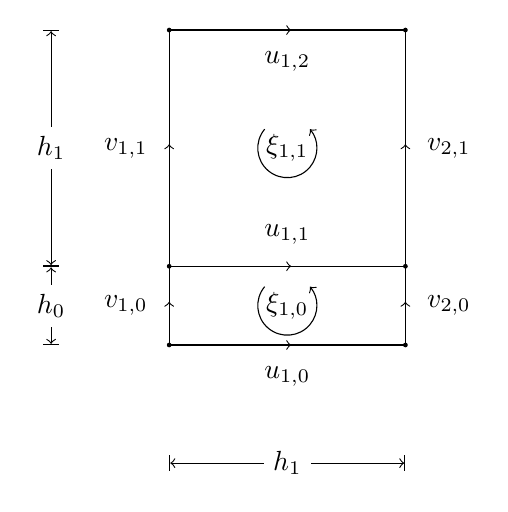
\begin{tikzpicture}
        % Draw scale
        \foreach \ia/\ib/\count in {0/1/0, 1/4/1} {
            \draw [|<->|] (-0.5,\ia) -- (-0.5,\ib) node [midway,fill=white] {$h_\count$};
        }
        \foreach \ia/\ib/\count in {1/4/1} {
            \draw [|<->|] (\ia,-1.5) -- (\ib,-1.5) node [midway,fill=white] {$h_\count$};
        }
        % Draw lines
        \draw (1,0) -- (1,4);
        \draw (4,0) -- (4,4);
        \draw (1,1) -- (4,1);
        \draw (1,1) -- (4,1);
        \draw (1,0) -- (4,0);
        \draw (1,4) -- (4,4);
        % Six corner points
        \fill (1,0) circle (0.03);
        \fill (4,0) circle (0.03);
        \fill (1,4) circle (0.03);
        \fill (4,4) circle (0.03);
        \fill (1,1) circle (0.03);
        \fill (4,1) circle (0.03);
        % Draw v
        \foreach \x/\i in {1/1} {
            \foreach \y/\j in {0.5/0, 2.5/1} {
                \draw [->] (\x,\y) -- (\x,\y+0.05);
                \node[left=1ex] at (\x,\y) {$v_{\i,\j}$};
            }
        }
        \foreach \x/\i in {4/2} {
            \foreach \y/\j in {0.5/0, 2.5/1} {
                \draw [->] (\x,\y) -- (\x,\y+0.05);
                \node[right=1ex] at (\x,\y) {$v_{\i,\j}$};
            }
        }
        % Draw u
        \foreach \x/\i in {0/0, 4/2} {
            \foreach \y/\j in {2.5/1} {
                \draw [->] (\y,\x) -- (\y+0.05,\x);
                \node[below=1ex] at (\y,\x) {$u_{\j,\i}$};
            }
        }
        \foreach \x/\i in {1/1} {
            \foreach \y/\j in {2.5/1} {
                \draw [->] (\y,\x) -- (\y+0.05,\x);
                \node[above=1ex] at (\y,\x) {$u_{\j,\i}$};
            }
        }
        % Draw xi
        \foreach \x/\i in {2.5/1} {
            \foreach \y/\j in {0.5/0, 2.5/1} {
                \draw [->] (\x,\y) ++(140:0.375) arc (-220:40:0.375);
                \node at (\x,\y) {$\xi_{\i,\j}$};
            }
        }
    \end{tikzpicture}
    \caption{Convection through $u_{1,1}$.}
    \label{fig:convectionExample}
\end{figure}

Because $u_{1,1}$ is a strictly horizontal line segment, we need not to consider the horizontal component of the convection through this line segment. Computing the mean vertical velocity in the plane below $u_{1,1}$ and multiplying it by $\tilde{\psi}_{1,0}$, we have
\begin{equation}
    -\frac{1}{2} \left( \frac{v_{1,0}}{h_0} + \frac{v_{2,0}}{h_0} \right) \tilde{\psi}_{1,0}
    \label{eq:planeBelow}
\end{equation}
For the plane above $u_{1,1}$, we have
\begin{equation}
    -\frac{1}{2} \left( \frac{v_{1,1}}{h_1} + \frac{v_{2,1}}{h_1} \right) \tilde{\psi}_{1,1}
    \label{eq:planeAbove}
\end{equation}
The average of Equations \eqref{eq:planeBelow} and \eqref{eq:planeAbove} multiplied by the length of $u_{1,1}$ yields the convection accross $u_{1,1}$:
\begin{flalign}
    & & \mathclap{\frac{1}{2} \left[ -\frac{1}{2} \left( \frac{v_{1,0}}{h_0} + \frac{v_{2,0}}{h_0} \right) \tilde{\psi}_{1,0} - \frac{1}{2} \left( \frac{v_{1,1}}{h_1} + \frac{v_{2,1}}{h_1} \right) \tilde{\psi}_{1,1} \right] h_1} && \\
    & \text{or} & \mathclap{-\frac{h_1}{4 h_0} \left( v_{1,0} + v_{2,0} \right) \tilde{\psi}_{1,0} - \frac{h_1}{4 h_1} \left( v_{1,1} + v_{2,1} \right) \tilde{\psi}_{1,1}} &&
\end{flalign}
The multipliplication by the length of $u_{1,1}$ is neseccary because the momentum equation is as a 1-form equation. That is, all terms of the momentum equation must ultimately be expressed as inner-oriented 1-cochains. Repetition of the above procedure for all line segments $u_{i,j}$ and $v_{i,j}$ yields
\begin{equation}
    \mbox{convection}
    =
    \begin{bmatrix}
    - \frac{\tilde{h}_1}{4 \tilde{h}_0} \left( v_{1,0} + v_{2,0} \right) \psi_{1,0} - \frac{\tilde{h}_1}{4 \tilde{h}_1} \left( v_{1,1} + v_{2,1} \right) \psi_{1,1} \\[10pt]

    - \frac{\tilde{h}_2}{4 \tilde{h}_0} \left( v_{2,0} + v_{3,0} \right) \psi_{2,0} - \frac{\tilde{h}_2}{4 \tilde{h}_1} \left( v_{2,1} + v_{3,1} \right) \psi_{2,1} \\[10pt]

    - \frac{\tilde{h}_1}{4 \tilde{h}_1} \left( v_{1,1} + v_{2,1} \right) \psi_{1,1} - \frac{\tilde{h}_1}{4 \tilde{h}_2} \left( v_{1,2} + v_{2,2} \right) \psi_{1,2} \\[10pt]

    - \frac{\tilde{h}_2}{4 \tilde{h}_1} \left( v_{2,1} + v_{3,1} \right) \psi_{2,1} - \frac{\tilde{h}_2}{4 \tilde{h}_2} \left( v_{2,2} + v_{3,2} \right) \psi_{2,2} \\[10pt]

    - \frac{\tilde{h}_1}{4 \tilde{h}_2} \left( v_{1,2} + v_{2,2} \right) \psi_{1,2} - \frac{\tilde{h}_1}{4 \tilde{h}_3} \left( v_{1,3} + v_{2,3} \right) \psi_{1,3} \\[10pt]

    - \frac{\tilde{h}_2}{4 \tilde{h}_2} \left( v_{2,2} + v_{3,2} \right) \psi_{2,2} - \frac{\tilde{h}_2}{4 \tilde{h}_3} \left( v_{2,3} + v_{3,3} \right) \psi_{2,3} \\[10pt]

    \frac{\tilde{h}_0}{4 \tilde{h}_0} \left( u_{0,1} + u_{0,2} \right) \psi_{0,1} + \frac{\tilde{h}_0}{4 \tilde{h}_1} \left( u_{1,1} + u_{1,2} \right) \psi_{1,1} \\[10pt]

    \frac{\tilde{h}_1}{4 \tilde{h}_1} \left( u_{1,1} + u_{1,2} \right) \psi_{1,1} + \frac{\tilde{h}_1}{4 \tilde{h}_2} \left( u_{2,1} + u_{2,2} \right) \psi_{2,1} \\[10pt]

    \frac{\tilde{h}_2}{4 \tilde{h}_2} \left( u_{2,1} + u_{2,2} \right) \psi_{2,1} + \frac{\tilde{h}_2}{4 \tilde{h}_3} \left( u_{3,1} + u_{3,2} \right) \psi_{3,1} \\[10pt]

    \frac{\tilde{h}_0}{4 \tilde{h}_0} \left( u_{0,2} + u_{0,3} \right) \psi_{0,2} + \frac{\tilde{h}_0}{4 \tilde{h}_1} \left( u_{1,2} + u_{1,3} \right) \psi_{1,2} \\[10pt]

    \frac{\tilde{h}_1}{4 \tilde{h}_1} \left( u_{1,2} + u_{1,3} \right) \psi_{1,2} + \frac{\tilde{h}_1}{4 \tilde{h}_2} \left( u_{2,2} + u_{2,3} \right) \psi_{2,2} \\[10pt]

    \frac{\tilde{h}_2}{4 \tilde{h}_2} \left( u_{2,2} + u_{2,3} \right) \psi_{2,2} + \frac{\tilde{h}_2}{4 \tilde{h}_3} \left( u_{3,2} + u_{3,3} \right) \psi_{3,2} \\
    \end{bmatrix}
\end{equation}
